\section{Preiskovanje}

\subsection{Neinformirani preiskovalni algoritmi}

\subsubsection{Iskanje v sirino}

\subsubsection{iskanje v globino}

Izboljsave:
\begin{itemize}
    \item \textbf{Iskanje s sestopanjem}
    \item \textbf{depth-limited-search} (vnapej definiramo globino l (dolocimo preko domenskega znanja))
\end{itemize}

\subsubsection{iterativno poglabljanje}
problem gobinsko omejenega iskanja -> nastavitev meje l
Mejo l postopoma povecujemo za 1, dokler ne najdemo resitve.
% itemize without spacing
\begin{itemize}[noitemsep,topsep=0pt]
    \item \textbf{popolnost}: Da
    \item \textbf{optimalnost}: Da
    \item \textbf{casovna zahtevnost} $O(b^d)$
    \item \textbf{prostorska zahtevnost} $O(bd)$
\end{itemize}
Boljse od iskanja v globino/sirino

\subsubsection{dvosmerno iskanje}
Ideja: pognati vzporedni iskanji od zacetka do cilja in od cilja do zacetka.\\
Motivacija: \\ 

\textbf{Implemenatcija dvosmernega iskanja}

\begin{itemize}[noitemsep,topsep=0pt,leftmargin=*]
    \item ciljno vozlisce mora biti znano
    \item originalni problemski prostor preslikamo v dvosmerni prosto stanj
    E1, E2 dosegljiv iz E in S1,S2,S3 dosegljiv iz S
    (S,E) -> {(S1, E1), (S1,E2), (S2, E1), (S2, E2)...}
    Vozlisce (Si, Ei) je v dvosmernem prostur ciljo vozlisce ce velja E=S (soda dolzina na isto mesto pridemo iz obeh strani) ali S->E (liha pot sosednja)
\end{itemize}

\subsubsection{cenovno - optimalno iskanje}
\begin{itemize}[noitemsep,leftmargin=*,topsep=0pt]
    \item posplositev iskanja v sirino (iskanje v sirino je optimalno, ce so cene vseh povezav enake 1)\\
    \item dijkstra basically (sam do zadnga noda)
    \item https://stackoverflow.com/a/14587449
\end{itemize}


\subsubsection{Primerjava algoritmov}

$$
\begin{array}{|c|c|c|c|c|c|}
   \hline 
   \text{Kriterij} & \text{sirino} & \text{globino} & \text{omejitvijo globine} & \text{iterativno poglabljanje} & \text{dvosmerno iskanje}\\
   \hline
\end{array}
$$


\subsection{Informirani preiskovalni algoritmi}

\subsubsection{hevristicno preiskovanje}
ideja: preiskovanje usmerjamo z dodatnim znanjem (ocenitven funcija za obetavnost vozlisca)\\
\textbf{hevristika} je ocenitvena funkcija za obetavnost vozlisca\\
- \green{optimisticna/dopustna}: $h(n) \leq h^*(n)$ ($h^*$ je optimalna ocena)\\
- \green{optimalna}: $h(n) = h^*(n)$\\
- \green{pesimisticna}: $h(n) \geq h^*(n)$\\


\subsubsection{pozresno preiskovanje/ greedy best-first search}
$h(n)$ hevristicna ocena\\
vrednotenje vozlisca $f(n)=h(n)$
hevristicna ocena ... npr manhattan distance (zracna razdalja)

\begin{itemize}[noitemsep,topsep=0pt,leftmargin=*]
    \item \textbf{popolnost} (ali najde vedno resitev): Ne
    \item \textbf{optimalnost}: Ne
    \item \textbf{casovna zahtevnost} $O(b^m)$, kjer je m najvecja globina drevesa
\end{itemize}

\subsubsection{A*}
A* is informed version of \textbf{dijkstra} (uses heuristics and pq)\\
Vozlisca vrednotimo: $f(n)=g(n)+h(n)$\\ 
$g(n)$ cena poti do n (znano),\\ 
$h(n)$ cena od n do najblizjega cilja (ocena)\\
\textbf{prioritetna vrsta} (max glede na f(n))
Basically dijkstra + h(n) (A* is basically an informed variation of Dijkstra.
)
\begin{itemize}[noitemsep,topsep=0pt,leftmargin=*]
    \item \textbf{popolnost}: Da (ce ustreza pogoju \underline{dopustnosti})
    \item \textbf{optimalnost}: Da (ce ustreza pogoju \underline{dopustnosti}) 
    \item \textbf{casovna zahtevnost} $O(b^m)$, kjer je m najvecja globina drevesa
\end{itemize}


\subsubsection{IDA* (Iterative deepening A*)}
DFS with heuristics and iterative bound (value)\\

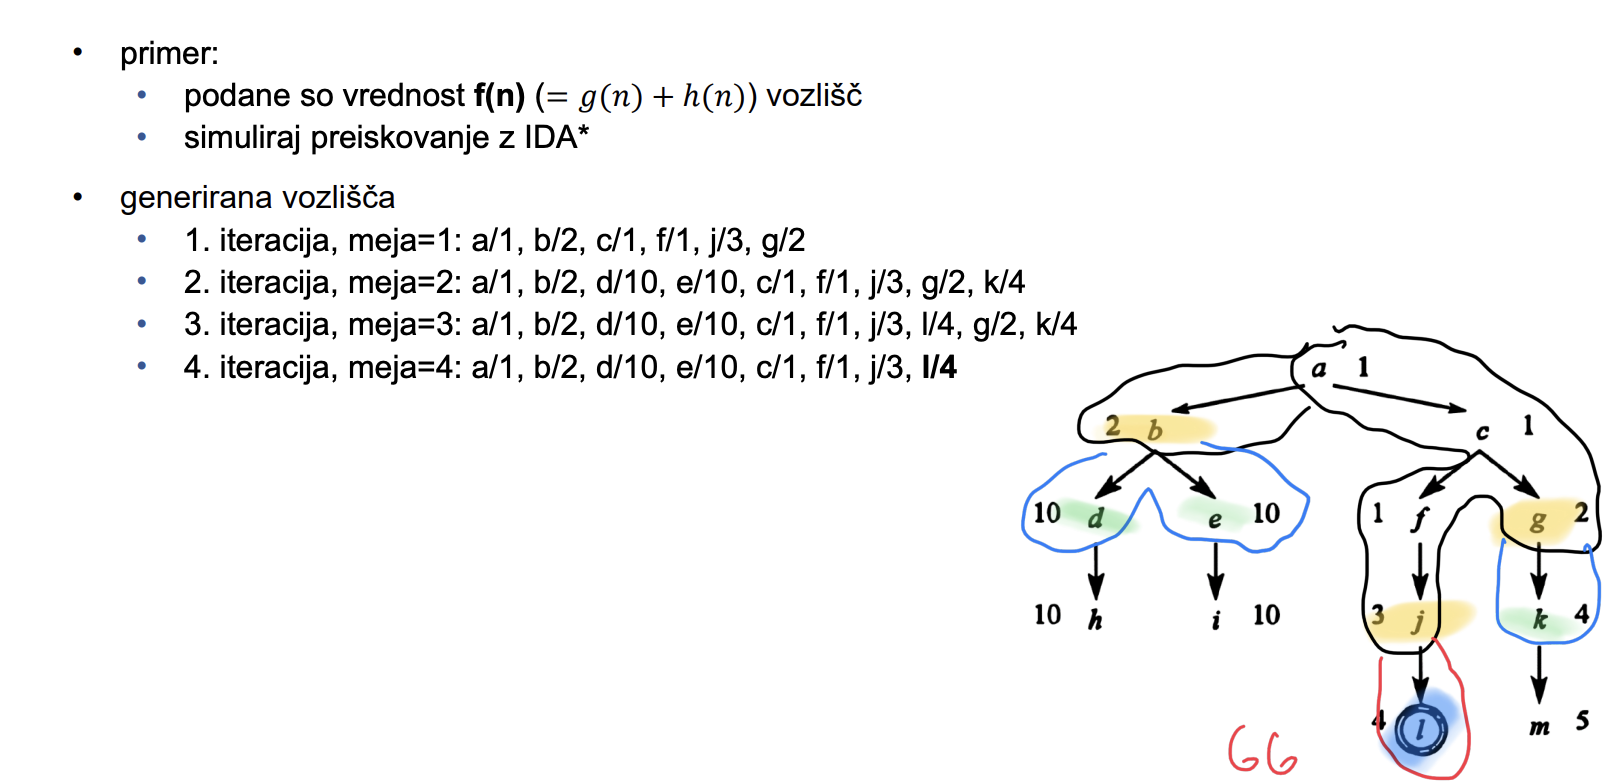
\includegraphics[width=6cm]{./images/ida*.png}

\textbf{Ucinkovitost}
\begin{itemize}[noitemsep,topsep=0pt,leftmargin=*]
    \item neucinkovit ce vozlisca raznolika f(n)
    \item prednost: ne hrani vec vseh vozlisc kot A*
    \item optimalen: ce razvija v prioritetnem vrsntem redu, h(n) mora biti \textbf{monotona|konsistentna} (h(n) skos pada) (posledicno tudi dopustna) $$h(n) \leq c(n,n') + h(n')$$ (h naslednjega vozlisca manjsi ker je blizji cilja)
    \item $\text{monotona} \rightarrow \text{dopustna}$ (proti primer h(n) = 0)
\end{itemize}


\subsubsection{Kakovost hevristicnih funkcij}
$$\begin{array}{|c|c|c|}
    \hline
    7 & 2 & 4 \\
    \hline 
    5 & & 6 \\
    \hline 
    8 & 3 & 1 \\
    \hline 
\end{array}\\$$
Primer igra 8 ploscic\\
-$h_1$: stevilo ploscic ki niso na pravem mestu (8)\\
-$h_2$: vsota manhattanskih razdalj ploscic do pravega mesta(3+1+2+2+2+3+3+2=18)\\
Kakovost h ocenimo z:\\
- stevilom generirarnih vozlisc\\
- z efektivnim faktorjem vejanja (koliko vozlisc N je algoritem generiral da je na globini d nasel resitev)\\

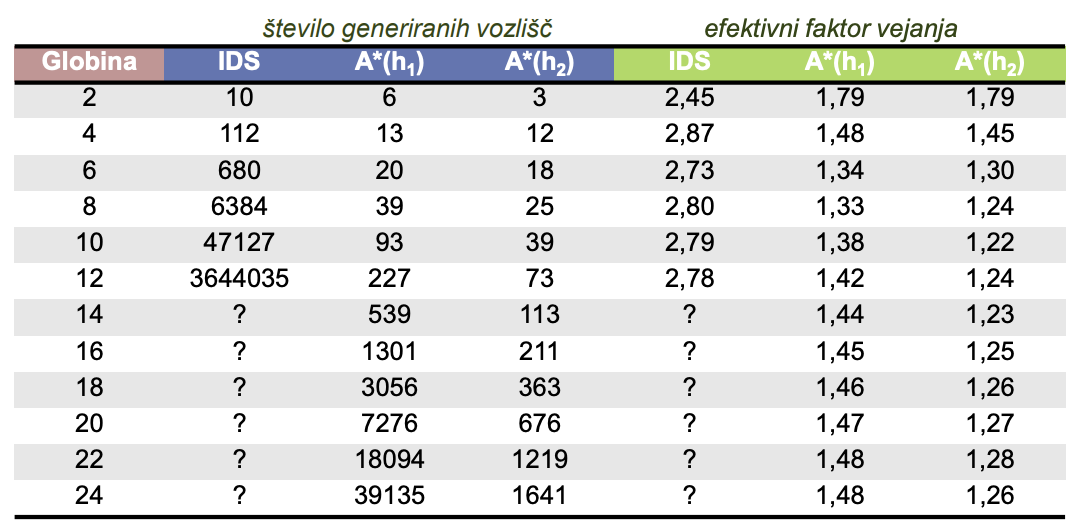
\includegraphics[width=6cm]{./images/kakovost-h(n).png}

Vidimo $h_2(n) \geq h_1(n) \forall n$ pravimo $h_2$ \textbf{dominira} $h_1$\\


\subsection{Lokalno preiskovalni algoritmi}

\subsubsection{Plezanje na hrib}
Ne pomnemo poti do cilja, ampak samo trenutno stanje\\
Koristni v primerih:\\
- ce nas zanima samo kakovost resitve (in ne pot do cilja)\\
- resevanje optimizacijskih problemov (kjer je podana \textbf{kriterijska funkcija} za oceno kakovosti resitve)\\

Prednosti:\\
- majhna poraba prostora\\

\textbf{Primer 4 kraljice na sahovnici}
- kriterijska funkcija: maksimiziramo - (minus) stevilo kraljic, ki se medsebojno napadajo

Tezave:
\begin{itemize}[noitemsep,topsep=0pt,leftmargin=*]
    \item lokalni maksimumi
    \item "rame, plaote" (kriterijska funkcija konstantna vrednost)
    \item grebeni (za plezanje navzgor je potreben sestop po pobocju grebena)
\end{itemize}

Resevanje iz lokalnih maksimumov:
\begin{itemize}[noitemsep,topsep=0pt,leftmargin=*]
    \item \textbf{koraki vstran}: ce ima naslednje stanje isto vrednost kriterijske funkcie, dovolimo premik v to stanje
    \item \textbf{stohasticno} plezanje na hrib: iz mnozice boljsih stanj, verjetnostno izberemo naslednje stanje (pri cemer upostevamo da imajo boljsa stanja vecjo verjetnost izbora)
    \item \textbf{nakljucni ponovni zagon}: veckrat pozeni plezanje na hrib iz nakljucnih stanj dokler ne najdes resitve
\end{itemize}

\subsubsection{Simulirano ohlajanje}
algoritem ki izvira iz metalurgije (ko je jeklo tekoce, so molekule v njem bolj gibljive; ko se ohlaja se strjuje in molekuele se umirjajo)
Analogija:\\
- generiramo nakljucne sosede trenutnega stanja\\
- ce najdemo \textbf{boljse stanje ga izberemo}\\
- ce najdemo \textbf{slabse stanje, ga izberemo z doloceno verjetnostjo}\\
- verjetnost izbire neoptimalnega stanja s casom pada (nizanje temperature)

\subsubsection{Lokalno iskanje v snopu}
Algoritem:\\
- v spominu hrani k aktualnih stanj namesto enega\\
- izberi k optimalnih stanj od sosedov aktualnih stanj\\
- ponavaljaj do ustavitnega pogoja 

\subsection{preiskovanje grafov AND/OR, nedeterministicno okolje}
Pomagajo resevati probleme z \textbf{dekompozicijo na manjse probleme}
Uporabnost:
\begin{itemize}[noitemsep,topsep=0pt,leftmargin=*]
    \item princip deli in vladaj
    \item iskanje v nedeterministicnih okoljih 
    \item igre med dvema nasprotnikoma s popolno informacijo (sah, dama)
    \item ekspertno resevanje problem
\end{itemize}
Primer graf dekompozicja v dva manjsa problema skozi g in f\\
\textbf{Resitveno drevo} je resitev AND/OR grafov\\
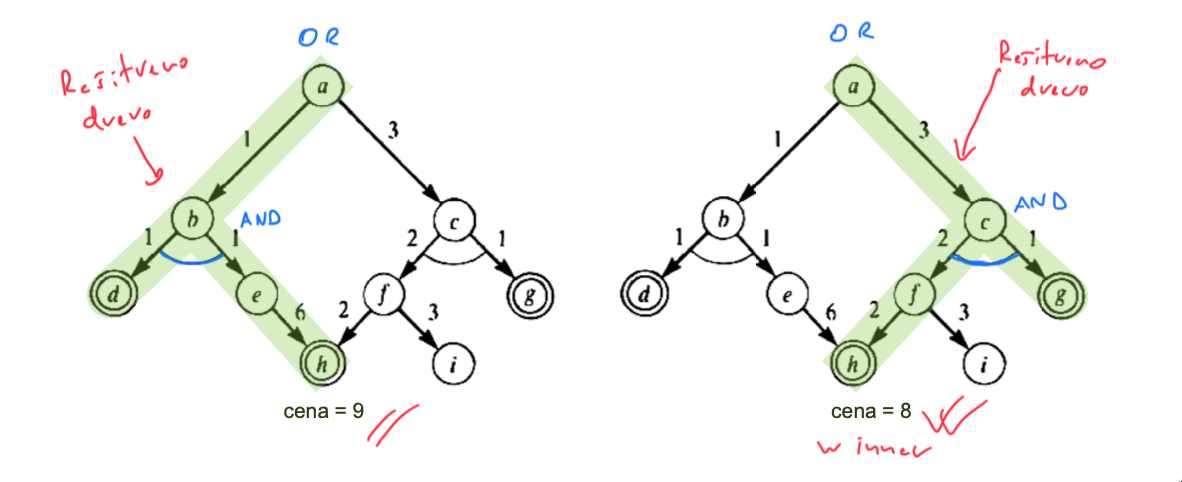
\includegraphics[width=6cm]{./images/resitveno-drevo.png}
\subsubsection{AO*}
Vozlisce \textbf{OR}: Razvijamo najbolj obetavno poddrevo, dokler njegova cena ne preseze alternativnega poddrevesa
Konec (AND vozlisca imajo v vsaki veji resitev, OR pa vsaj v eni)

\begin{itemize}[noitemsep,topsep=0pt,leftmargin=*]
    \item posplositev A* na grafe AND/OR
    \item \textbf{popoln in optimalen} $\Leftrightarrow$ h(n) ne precenjuje dejanske cene do cilja
\end{itemize}

Vsako vozlisce N ima:
\begin{itemize}[noitemsep,topsep=0pt,leftmargin=*]
    \item lokalno (dinamicno) \textbf{hevristicno oceno} \green{H(N)}
    \item lokalno (dinamico) vrednost \textbf{kriterijske funkcije} \green{F(N)}
    G(N) cena od predhodnika do trenutnega vozlisca
    $$F(N_i)=G(N_i)+H(N_i)=\textbf{cena}(N_{i-1},N_i)+H(N_i)$$
\end{itemize}
Dinamicna hevristicna ocena H(N) je \textbf{odvisna od tipa vozlisca}:
\begin{itemize}[noitemsep,topsep=0pt,leftmargin=*]
    \item za \green{liste}:
        \item H(N) = h(n)
        \item F(N) = G(N) + H(N) = cena(stars,N) + h(n)
    \item za \green{notranja vozlisca}:\\
    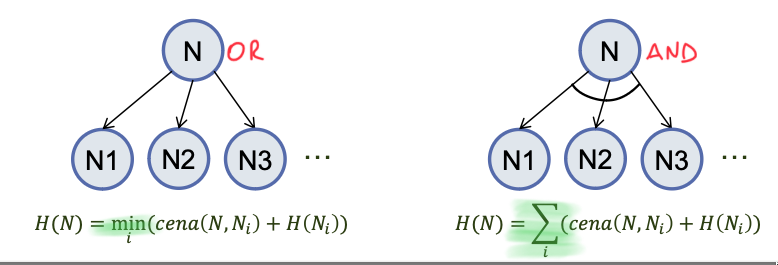
\includegraphics[width=6cm]{ao+.png}
\end{itemize}
\subsubsection{Preiskovanje v nedeterministicnem okolju:}
\textbf{Nedeterministican akcija} - ista akcija lahko obrodi razlicna ciljna stanja\\
Do resitve ni vec \textbf{poti} temvec \textbf{drevesa} (uporbljamo AND/OR grafe)\\
Vozsilca OR \textbf{mozne akcije}, vozlisca AND \textbf{vejanja v mozna stanja}, ki so rezultat nedeterministicnih akcij

\subsection{Preiskovanje brez informacij o stanju}
Okolja smo razdelili na \textbf{transparent} (agent lahko zazna popolno informacija) in \textbf{netransparentna} (brez informacije o stanju)\\
Kej ce imamo opravka z netraspranetim okoljem?\\
- izvajamo preiskovanje prostora \textbf{verjetnih} stanj in ne prostora \textbf{dejanskih} stanj\\
- izvajamo s postokopom omejevanja moznozsti kandidatnih stanj\

\subsection{Igranje iger}

\subsubsection{Predstavitev problema}

\subsubsection{algoritem MINIMAX}
- m globina
- b 

\subsubsection{Rezanje alfa-beta}
